\documentclass{article}

\usepackage[a4paper,margin=1.15in,footskip=0.25in]{geometry}

\usepackage[utf8]{inputenc}
\usepackage[english]{babel}
\usepackage{textpos}
\usepackage{textcomp}
\usepackage{amsmath}
\usepackage{amssymb}
\usepackage{amsfonts}
\usepackage{graphicx}
\usepackage{epstopdf}
\usepackage{algorithmic}
\usepackage{verbatim}
\usepackage{textcomp}
\usepackage{varwidth}
\usepackage[linesnumbered,ruled]{algorithm2e}

% Theorem
\newtheorem{theorem}{Theorem}

% lists
\usepackage{outlines}
\usepackage{enumitem}
\newenvironment{tight_enum}{
\begin{enumerate}[label=\alph*.]
\setlength{\itemsep}{0pt}
\setlength{\parskip}{0pt}
}{\end{enumerate}}

% \subsubsubsection{}
\setcounter{secnumdepth}{5}
\setcounter{tocdepth}{5}
\newcommand\simpleparagraph[1]{%
  \stepcounter{paragraph}\paragraph*{\theparagraph\quad{}#1}}

\usepackage{listings}
\usepackage{color}
\usepackage{xcolor}
\usepackage{mdframed}

\definecolor{dkgreen}{rgb}{0,0.6,0}
\definecolor{gray}{rgb}{0.5,0.5,0.5}
\definecolor{mauve}{rgb}{0.58,0,0.82}

% \usepackage{courier}
\lstset{%frame=tb,
language=C++,
aboveskip=3mm,
belowskip=3mm,
showstringspaces=false,
columns=flexible,
basicstyle={\small\ttfamily},
numbers=none,
numberstyle=\tiny\color{gray},
keywordstyle=\color{blue},
commentstyle=\color{dkgreen},
stringstyle=\color{mauve},
breaklines=true,
breakatwhitespace=true,
tabsize=3
}

%%%%%%%%% BEGIN DOCUMENT %%%%%%%%%
%%%%%%%%% BEGIN DOCUMENT %%%%%%%%%
%%%%%%%%% BEGIN DOCUMENT %%%%%%%%%

\begin{document}

\title{An optimization-inspired approach to parallel sorting}
\author{Team Metropolis: \\
		Jamshid 'James' Farzidayeri, JJ Lay, and Graham West}
\date{COMS 7900, Capstone}

\maketitle

\begin{abstract}
We present a novel method influenced by ideas in the field optimization to efficiently sort large amounts of data in parallel on a cluster of computing nodes. We describe in depth the different challenges which beset such a method, including distributing/importing files, locally sorting the data on each node, uniformly binning the data, and exchanging data between the nodes. We also present the results of several different timing tests applied to the method. These tests demonstrate how the method scales when the number of files and/or the number of nodes is increased. Finally, we summarize the the greatest challenges in implementing the method, as well as the components of the method which were the most successful. We conclude with a discussion on ways in which the method could be improved.
\end{abstract}


\tableofcontents


%%%%%%%%%%%%%
%%% NEW SECTION %%%
%%%%%%%%%%%%%
\section{The Method}


As our first project for COMS 7900, the objective was to develop a system that would use MPI and the Babbage cluster to read in a significant amount of raw data and output that data in sorted sections. The data consisted of 500 files each with 20 million lines of data points. Each data point contained a integer number with three floating point coordinates. The project must allow for the sorting of data by any of the coordinate columns of data points. Additionally, the project must output the sorted information using qsub and have the data stored in files listed from smallest to largest. Finally, the system must allow for testing the output for verification of the sorting and a method for process timing. After the assignment was distributed, the team members met to discuss and develop a brief outline of how the assignment would be handled. It was concluded that a prototype would be developed using Mat Lab, and the final project would use C++ with C MPI calls. It was at that time Graham began working with the Metropolis algorithm. As the project took shape JJ set up GitHub and provided Graham and James with additional GitHub training. JJ also set up the structure for how the code would be presented, including general outline of the main program's structure and the outline for different files needed. Then the team met and presented with Graham's Mat Lab prototyping. It was after the second meeting that work assignments began to be handed out and we agreed upon several variables and conventions. Several pieces of the C++ code were developed simultaneously. JJ worked on file I/O and distribution, Graham developed bin adapting, and James worked on sorting and data exchanging. The code was assembled and any remaining issues resolved. 




\subsection{Overview}


\subsubsection{Workflow}
We used C++ with C MPI calls

Used GitHub

Workflow description


\subsubsection{Variables and conventions}
%%% NOTE %%%
%%% NOTE %%%
% 1) be consistent with the indices:
% 2) say head node (not master node)
% 3) say worker (not node) whenever possible
%%% NOTE %%%
%%% NOTE %%%

Here we provide a helpful list of conventions, notations, and variable names used throughout this paper.

\begin{mdframed}[backgroundcolor=blue!20]
	Counts:
	\setlength\itemsep{0.1pt}
	\setlength\parskip{0.1pt}
	\begin{itemize}
		\setlength\itemsep{0.1pt}
		\setlength\parskip{0.1pt}
		\item $N$: number of nodes
		\item $W$: number of workers ($N-1$)
		\item $L$: number of lines to read per file
		\item $L_w$: number of lines on the $w$th worker
		\item $M$: max number of allowed time steps
	\end{itemize}
\end{mdframed}

\begin{mdframed}[backgroundcolor=blue!20]
	Indices:
	\setlength\itemsep{0.1pt}
	\setlength\parskip{0.1pt}
	\begin{itemize}
		\setlength\itemsep{0.1pt}
		\setlength\parskip{0.1pt}
		\item $m = 0, \cdots, M$ is the time step of the bin adaptation scheme (likely less than $M$)
		\item $n = 0, \cdots, W$ spans the nodes
		\item $w = 1, \cdots, W$ spans the workers
		\item $i = 0, \cdots, W$ spans the bin edges/indices
		\item $j = 1, \cdots, W$ spans the bin counts (this will occasionally subscript binI/E as well)
		\item $\ell_w = 0, \cdots, L_w-1$ spans the lines on the $w$th worker
		\item $k = 0, \cdots, 3$ is the data column being sorted
	\end{itemize}
\end{mdframed}

\begin{mdframed}[backgroundcolor=blue!20]
	Variables:
	\setlength\itemsep{0.1pt}
	\setlength\parskip{0.1pt}
	\begin{itemize}
		\setlength\itemsep{0.1pt}
		\setlength\parskip{0.1pt}
		\item $\textrm{data}^w_{4\ell+k}$: data point on $\ell$th line and $k$th column (0 indexed)\\ on the $w$th worker (1 indexed)
		\item $\textrm{binE}^m_j$: bin edges (0 indexed) at time step $m$
		\item $\textrm{binI}^{w,m}_j$: bin indices on worker $w$ (0 indexed)
		\item $\textrm{binC}^{w,m}_j$: bin counts on worker $w$ (1 indexed w.r.t. $w$) at time step $m$
		\item $\textrm{binC}^{0,m}_j$: bin counts on head node (sum of worker binC's) at time step $m$
	\end{itemize}
\end{mdframed}


% JJ
\subsection{File I/O}

There are two main steps in the initial file I/O phase. The first step is to identify the candidate data files and assign them to worker nodes. The second part is for the workers to import the data files into memory.



\subsubsection{Distributing files}

Hello worled

\subsubsection{Importing files}

Worker nodes import files using the \texttt{getline} function to read each line individually into a \texttt{string}. Fields are then parsed from the string based on their positions.

\begin{tabular}{l l l l}
\textbf{Field} & \textbf{Starting Pos} & \textbf{Ending Pos} & \textbf{Data Type} \\
Index &  0 & 12  & Ignored \\
X     & 13 & 35  & double  \\
Y     & 36 & 54  & double  \\
Z     & 55 & EOL & double \\
\end{tabular}

The \texttt{Index} field is calculated using the value from the filename and a maximum number of rows in each file of 20000000. The starting index value for a file is:

$I_0 = (Filename - 1) * 20000000$

The index is then incremented for each row and used in lieu of the value from the file. By storing the index as a double, the need for a complex C \texttt{struct} is avoided, and the data can be stored in a one-dimensional array of doubles.




% JF
\subsection{Sorting}
In this section we address the two options for sorting the data. Since the majority of the groups are using qsort or some variation of that. We felt it would be interesting to have some alternative options for comparison for the class. Therefore we offer two options while using our process: a linked list insertion sort and bubble sort. Both options require the user pass information in the following format. 
% here's how to insert code into LaTeX
\begin{lstlisting}
            void LL_sort(double myArray[], int rows, int cols, int sortThisColumn)
\end{lstlisting}
Each option first uses the value in 'sortThisColumn' to determine which column the user is requesting the sort on. Both options also make modifications to the existing 'myArray[]'. The rows and column are used during the iteration process to determine the 'shape' of the array during iteration. The limiting factor for both options is that the user is currently restricted to just the four columns. However, the function could be easily modified the accept more columns.
\subsubsection{Linked list insertion sort}
The better of our two options by a significant margin is or linked list insertion sort. Inside this function is a one directional singly linked list made with the following node structure.
\begin{lstlisting}
                                    struct Node{
	                                    double ll_location;
	                                    double ll_x;
	                                    double ll_y;
	                                    double ll_z;
	                                    struct Node *next;
                                    };

\end{lstlisting}
The function initializes the linked with the first data point in the myArray[]. Then inserts each additional piece of data from myArray[] into the linked list using the traditional head, current, and previous pointer methods. After the method has iterated through all the data in myArray[] and has a now sorted linked list,  then the data is placed back into myArray[] and exits the program.
\subsubsection{Bubble sort}
This function is by far the weaker of the two options and considered one of the least desirable of all sort functions. However, it is quite easy to implement, very robust, requires no additional large memory sections, and extremely reliable. This method simply sorts in place using the classic bubble sort process below.
\begin{lstlisting}
           for (int iii = 0 ; iii < (rows);iii++){
		        for(int jjj=0; jjj<(rows-stop); jjj++){
			            if(myArray[cols*jjj+sortByThisColumn]>
			                myArray[cols*(jjj+1)+sortByThisColumn]){
				                //perform swap
\end{lstlisting}

Although this will not be used as part of our regular process, we are interested in seeing how poorly it performs compared to other algorithms. This method does does not attempt to resort the 'last' space of the previous iteration. This is a slight reduction in the $N^2$ average that is usually expected from bubble sort methods. 


% GW
\subsection{Binning}
% This is where the optimization stuff is
We now discuss the optimization-inspired portion of the method. It has optimization properties since we need to find the bin edges such that we maximum the uniformity of the distribution. However, it is a constrained form of optimization since the bin edges must always maintain the relation
\begin{equation}
	\textrm{binE}^m_i < \textrm{binE}^m_{i+1}
\end{equation}
As we will see, the way we construct our adaptation formulae ensures that this constraint is always met.

\subsubsection{Data binning w/ binary search}
Since we use an iterative scheme to adjust the bin edges through time, we use as an initial condition/approximation equally-spaced bin edges between the global min and max of the data. Now, since each worker could theoretically have millions of data points, repeatedly looping through the data to find the bin in which each point lies would be inefficient. As such, we use the fact that the data is sorted to expedite the process significantly by using binary search. Now, each worker will have the same bin edges $\textrm{binE}^m_i$ (where $i = 0, \cdots, W$), but the the location of the edges with respect to the data indices on each worker will likely be quite different if the data distribution across workers varies. With this in mind, for each worker, we search for the data indices at which each bin edge lies, giving us the new variables $\textrm{binI}^{w,m}_i$ (note the superscript $w$, indicating that each worker has its own unique set of bin indices). To do this, we search for the index $\ell$ such that
\begin{equation}
	\textrm{data}^w_{4\ell+k} < \textrm{binE}^m_i < \textrm{data}^w_{{4(\ell+1)+k}}
\end{equation}
giving $\textrm{binI}^{w,m}_i = \ell+1$. We also set $\textrm{binI}^{w,m}_0 = 0$ and $\textrm{binI}^{w,m}_W = L_w$. We then calculate $\textrm{binC}^{w,m}_j$:
\begin{equation}
	\textrm{binC}^{w,m}_j = \textrm{binI}^{w,m}_j - \textrm{binI}^{w,m}_{j-1}, \quad j = 1, \cdots, W
\end{equation}
Lastly, all workers send their bin counts to the head node and we calculate the total bin counts:
\begin{equation}
	\textrm{binC}^{0,m}_j = \sum_{w=1}^{W} \textrm{binC}^{w,m}_j, \quad j = 1, \cdots, W
\end{equation}


\subsubsection{Stopping criterion: the uniformity metric}
Once the head node has calculated the total bin counts, it then determines how uniformly the data distributed across the bins:
\begin{equation}
	U^m = \textrm{max} \bigg( \dfrac{\textrm{binC}^{0,m}_{\textrm{max}} - \textrm{binC}^{0,m}_{\textrm{avg}}}{\textrm{binC}^{0,m}_{\textrm{avg}}}, \dfrac{\textrm{binC}^{0,m}_{\textrm{avg}} - \textrm{binC}^{0,m}_{\textrm{min}}}{\textrm{binC}^{0,m}_{\textrm{avg}}} \bigg)
\end{equation}
If $U$ is below a set threshold (usually $\approx 0.1$), then the the data distribution is deemed to be uniform in the sense that each worker will have within $\approx 10\%$ of the average data per worker; thus sorting on each worker will take roughly equal time.


\subsubsection{Adapting bin edges}
If the data is not uniform in the first step, we move on to adapt the interior bin edges ($i = 1, \cdots, W-1$):
\begin{equation}
	\begin{split}
		\Delta C & = 2.0 ( \textrm{binC}^{0,m}_{i+1} - \textrm{binC}^{0,m}_i ) / ( \textrm{binC}^{0,m}_{i+1} + \textrm{binC}^{0,m}_i ) \\
		\Delta B & = \textrm{binE}^m_{i+1} - \textrm{binE}^m_i \\
		\textrm{binE}^{m+1}_i & = \textrm{binE}^m_i + \alpha \Delta C \Delta B
	\end{split}
\end{equation}
where $0 < \alpha < 0.5$. Each of these terms is designed the allow the bins to adapt the maximum amount possible without the bin edges becoming out of order. The quantity $\Delta B$ scales the maximum change to be within the current bin width. The quantity $0 \le \Delta C \le 1$ is a type of normalized gradient which will direct the bin edges toward regions with higher density. Lastly, $\alpha$ is a form of rate constant. It must remain less than 0.5 to maintain the constraint. It is usually set between 0.25-0.475.

\subsubsection{Prototyping in MATLAB}
Prior to our implementation in C++, we prototype the adaptation scheme in MATLAB as a proof of concept. For these tests, we read 1000 lines from one of the provided data files and applied the adaptive binning scheme to it, varying the number of nodes, iterations, and the value of $\alpha$.
\begin{figure}[!htb]
	\centering
	\vspace{-5pt}
	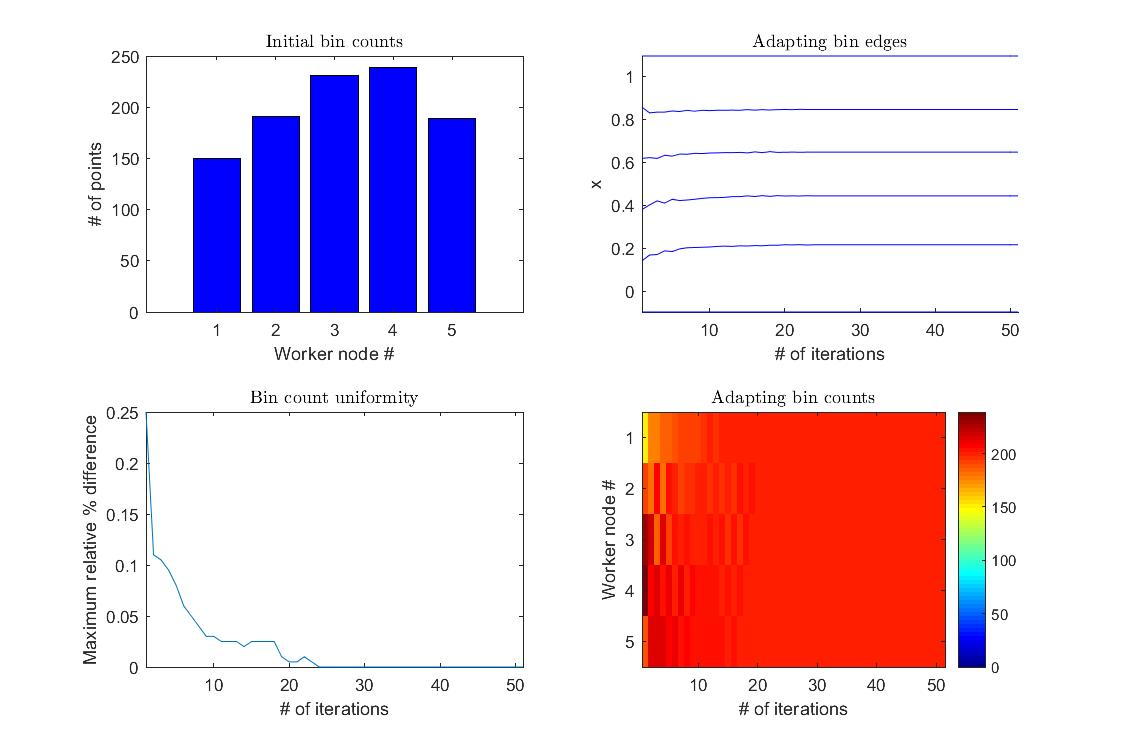
\includegraphics[scale = 0.25]{AdaptiveBinning_5Nodes_1000Lines_0475alpha}
	\vspace{-10pt}
	\caption{5 nodes, 1000 data points, $\alpha = 0.475$}
	\label{5,0.475}
\end{figure}
\begin{figure}[!htb]
	\centering
	\vspace{-5pt}
	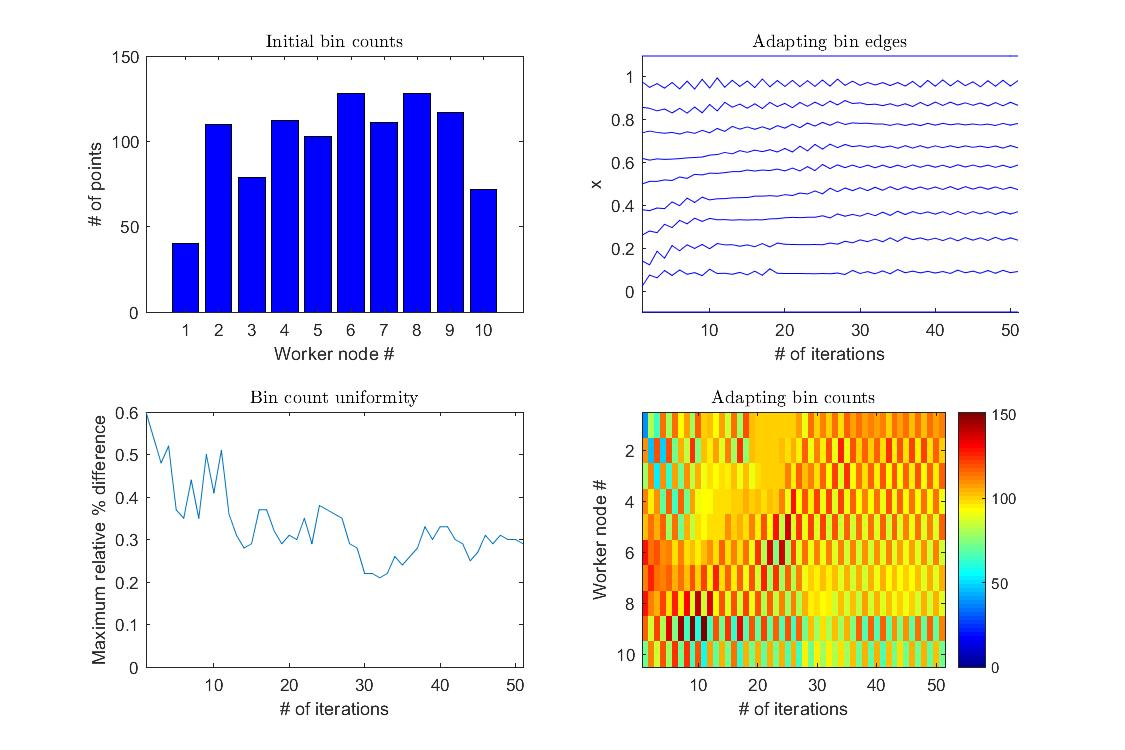
\includegraphics[scale = 0.25]{AdaptiveBinning_10Nodes_1000Lines_0475alpha}
	\vspace{-10pt}
	\caption{10 nodes, 1000 data points, $\alpha = 0.475$}
	\label{10,0.475}
\end{figure}
\begin{figure}[!htb]
	\centering
	\vspace{-5pt}
	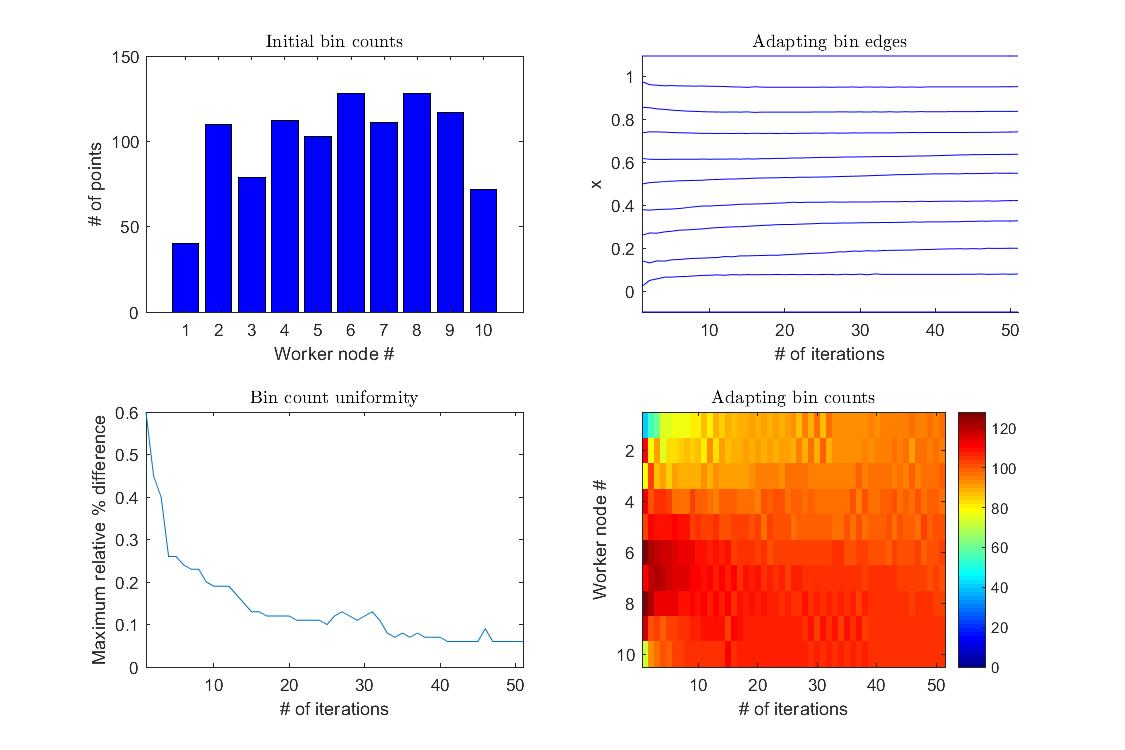
\includegraphics[scale = 0.25]{AdaptiveBinning_10Nodes_1000Lines_0250alpha}
	\vspace{-10pt}
	\caption{10 nodes, 1000 data points, $\alpha = 0.25$}
	\label{10,0.250}
\end{figure}

As can be seen from the Figure \ref{5,0.475}, with $W=5$ and $\alpha=0.475$, the method converges to a highly uniform distribution in roughly 20 steps. However, when increasing the number of workers to 10 (Figure \ref{10,0.475}), the method struggles to converge in the same amount of time. This problem arises because adding more workers adds more bin edges. Since the test only uses 1000 data points, then there is only an average of 100 points per bin, which is not sufficiently smooth for the method to perform at its optimal level. As such, we must decrease $\alpha$ so that we can remove the wild oscillations present in the plots. This is what Figure \ref{10,0.250} demonstrates. Though it still does not converge quite as fast as the 5 worker test, it is sufficiently better than the second test.

These tests demonstrate two general rules which describe the performance of the method. First, the method performs better (faster convergence, less oscillations) with more data since altering the bin edges on average won't have as drastic an effect on the bin counts. Also, the method performs worse (slower convergence, possible oscillatory behavior) with more workers (i.e., bin edges). There are two reasons for this. First, relating to the previous rule, since more granular divisions of the data counter the positive effects that large amounts of data have on performance. This being said, in practice, this effect is not significant when dealing with millions or billions of data points because no practical number of workers can make the data significantly granular. Second, since we use only a local bin updating scheme (a form of normalized gradient of the bin counts), the bin edges near the boundary of the data range do not have much room to move since the interior bin edges must move first (since we must maintain the constraint). Consequently, this makes our method susceptible to very poor performance if there is an outlier in the data, because there will be a large number of bin edges between the outlier and the rest of the data which cannot move until some data is propagated toward them. A clear improvement which could be made to the method would be to replace the local bin count gradient with a global analogue (whicj still maintains the constraint, of course).





% JF
\subsection{Exchanging data}
The exchanging data process for our design includes two steps: Data swap and Clean up. This is to allow flexibility in the main program during its implementation of the functions. 
\subsubsection{Data swap}
When this function is called, it uses a from/to process. Meaning that given the following set of options it will transfer a specific set of data from one node to another. 
\begin{lstlisting}
 void swapArrayParts(double *pmyArray[], int *rowPTR , int *colPTR, int myrank, int numranks, int *binIPTR, int fromWho, int toWho)        
\end{lstlisting}
The first thing the process does is pass information regarding the length of the data to be received from the array. If the node that called the function is considered 'fromWho' it will pass its binI information to the node who called the function as the 'toWho'. At this point, the node who is 'toWho' creates a temporary array that is large enough to fit both the current set of data plus the additional set of data it is about to receive. After that is completed the node 'fromWho' then passes the pointer to the beginning of the data point in pmyArray where the node 'toWho' begins it's length of data to transfer. Here the node who is considered 'fromWho' will exit the function and the node who is 'toWho' will simply insert the data from its current pmyArray into the temporary array. Then in the remaining spaces inserts the information it just received from 'fromWho'. Finally, the 'toWho' node will increase the number of rows to include the additional data points. Then 'toWho' exits the function. At this point, the 'fromWho' node still has all of its original data and the 'toWho' node now has its original data plus the additional data sent over from the 'fromWho' node. Since this is a one to one transfer, it can be implemented in anyway the main program chooses. For the purposes of our group's needs we choose to have one node send all of its information to each other then increment through all nodes in the following method.
\begin{lstlisting}
                for( fromWho = 1; fromWho < numNodes; fromWho++ ){
                    for( int toWho = 1; toWho< numNodes; toWho++){
                        if(toWho!=fromWho){
                            if(myRank ==toWho || myRank ==fromWho){
                                perform swapArrayParts
\end{lstlisting}
\subsubsection{Cleanup}
Once this method is complete each node will have all the information from each other node appended to the end of their existing array. However, each node will still have the information that it has passed to others and will now need to remove from their own array. This is where the cleanUp function is utilized. Whenever a function calls cleanUp it will need to receive the following parameters.
\begin{lstlisting}
                void cleanUp(double *pmyArray[], int *rowPTR , int *colPTR, int myrank, int numranks, int *binIPTR)
\end{lstlisting}
CleanUp first uses the information in '*binIPTR' to determine the amount and locations of the data that was given to other nodes and the amount of information it should retain inside its array. Then we malloc a temporary array with the correct size. The information that should be kept is inserted into the temporary array while excluding the data that should not be included. Then '*pmyArray[]' is pointed to the beginning of the temporary array and the row size is adjusted to reflect the new and correct size of the node's array. The node now exits the function with the correct size and information however the data is no longer sorted and a new sort must be completed. This function must be called individually for all nodes used in the swapArrayParts method. 


%%%%%%%%%%%%%
%%% NEW SECTION %%%
%%%%%%%%%%%%%
\section{Performance}

JJ's performance data sections go here



%%%%%%%%%%%%%
%%% NEW SECTION %%%
%%%%%%%%%%%%%
\section{Conclusions}
We will now conclude with two discussions on 1) the most difficult and most successful aspects of our method and 2) ways of improving the both the method's performance/efficiency and our workflow as a group.

\subsection{Challenges and successes}


\subsection{Future work}



%%%%%%%%%%%%%%%
%%%%% THE END %%%%%
%%%%%%%%%%%%%%%


\end{document}





